\documentclass[12pt,a4paper]{article}
\usepackage[utf8]{inputenc}
\usepackage[T1]{fontenc}
\usepackage{fontspec}
\usepackage[polish]{babel}
\usepackage{amsmath}
\usepackage{graphicx}
\usepackage[table,xcdraw]{xcolor}
\usepackage{hhline}
\usepackage{placeins}
\usepackage[margin=0.6in]{geometry}
\usepackage{appendix}
\usepackage{colortbl}
\usepackage{physics}
\usepackage{float}
\usepackage{datetime}
\usepackage{hyperref}

\title{Praca Domowa Termodynamika i Fizyka Statystyczna R 2021/2022}
\author{Kacper Cybiński}
% \newdate{date}{28}{01}{2022}
% \date{\displaydate{date}}
\date{\today}
\setlength\parindent{0pt}

\newcommand{\com}[1]{{\color{red} #1}}

\newcommand{\link}[2]{{\color{cyan} \href{#1}{#2}}}

\renewcommand{\emph}{\textbf}

\begin{document}

\maketitle

\section{Zadanie 2}

\begin{figure}[h!]
    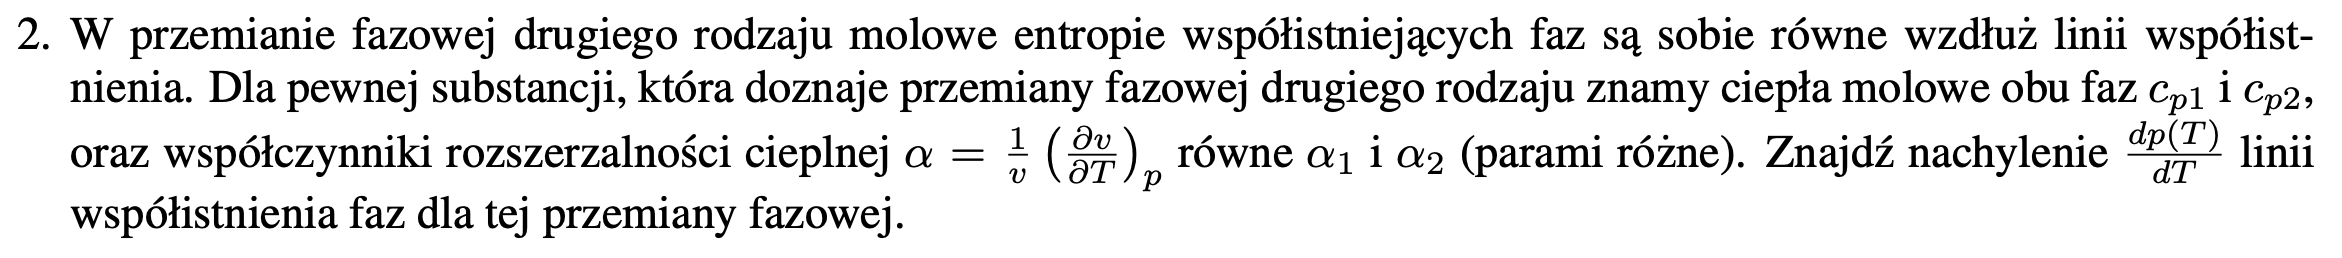
\includegraphics[width=\linewidth]{z2.png}
\end{figure}

\section{Rozwiązanie}

Zauważmy na początku, że jest to przemiana drugiego rodzaju, więc znany z wykładu wzorek nie zadziała (plus dostaniemy dla niego $\frac{0}{0}$).
    Wiadomo jednak, że mamy równość entropii molowych dla obu faz, to znaczy:
    \[s_1=s_2\]
    Skoro tak, to zachodzi również:
    \[ds_1=ds_2\]
    Załóżmy, że entropia molowa jest funkcją ciśnienia i temperatury.
    Wówczas mamy równość:
    \[ds=\left(\frac{\partial s}{\partial T}\right)_pdT+\left(\frac{\partial s}{\partial p}\right)_T dp\]
    Z definicji $\left(\frac{\partial s}{\partial T}\right)_p=c_p$, natomiast z relacji Maxwella mamy, że
    $\left(\frac{\partial s}{\partial p}\right)_T=-\left(\frac{\partial V}{\partial T}\right)_p=-\alpha v$.
    Czyli możemy zapisać:
    \[\frac{1}{T}c_{p1}dT-\alpha_1v_1dp=\frac{1}{T}c_{p2}dT-\alpha_2v_2\]
    \[(\alpha_1v_1-\alpha_2v_2)dp=\frac{1}{T}(c_{p1}-c_{p2})dT\]
    A stąd dostajemy szukany wynik:
    \[\dv{p}{T}=\frac{c_{p1}-c_{p2}}{T(\alpha_1v_1-\alpha_2v_2)}\]
    Ale skoro entropie są sobie równe to ze wzoru Clausiusa-Claperyona wnioskujemy, że $v_1=v_2$.
    Czyli ostatecznie:
    \[\dv{p}{T}=\frac{c_{p1}-c_{p2}}{Tv(\alpha_1-\alpha_2)}\]


\end{document}